\chapter{Oasis Local Db}
\label{ch:Db}
In this chapter we describe the Oasis Local Db.
The Oasis Local Db is used for storing the data, which is used by the GIRAF applications.
The database schema, which the Oasis Local Db is based upon, is described in Section \vref{sec:OasisSchema}.
The structure of SQLite used on the Android Platform is described in Section \vref{sec:OasisStructure}.
Finally the implementation of the Oasis Local Db on the Android system is described in Section \vref{sec:dbImp}.

\section{Database Schema}
\label{sec:OasisSchema}
The Oasis Local Db Schema is developed in cooperation with Savannah.
The reason for this is to alleviate the complexities that could occur during a synchronization of the Oasis Local Db and Savannah.

The central point of the Oasis Local Db schema is the AuthUsers table.
This table contains all the user id's and their certificates.
A user in the Oasis Local Db can be either a profile or a department and therefore a role is stored as well to differetiate the two.

The Oasis Local Db schema for the profiles and departments are a simple model representing a kindergarden like Birken or a school like Egebakken.
This means that a profile can either be a child or guardian.
The Oasis Local Db supports the possibility to associate profiles to each other in order to allow a child to guardian relation.
The profiles can be attached to one or more departments, and a department can be related to one or more sub departments.

An important part of the system for the guardians is the ability to access different kinds of media on the tablets.
Therefore media can be stored in the Oasis Local Db along with information about who has access to them.
A media can be owned by either a profile or a department, and the owner has the ability to decide who should have access to the media.
The Oasis Local Db schema also allows the user to adds tags to media, these tags can be used to identify the media.

Another important part of the system is the ability to control appplications.
From the users viewpoint it consists of deciding which applications should be accessible and from the developers viewpoint it is a way of storing application settings for a profile.

The Oasis Local Db schema can be seen in figure \autoref{fig:localDatabaseDesign}.

\begin{figure}[htbp]
	\centering
		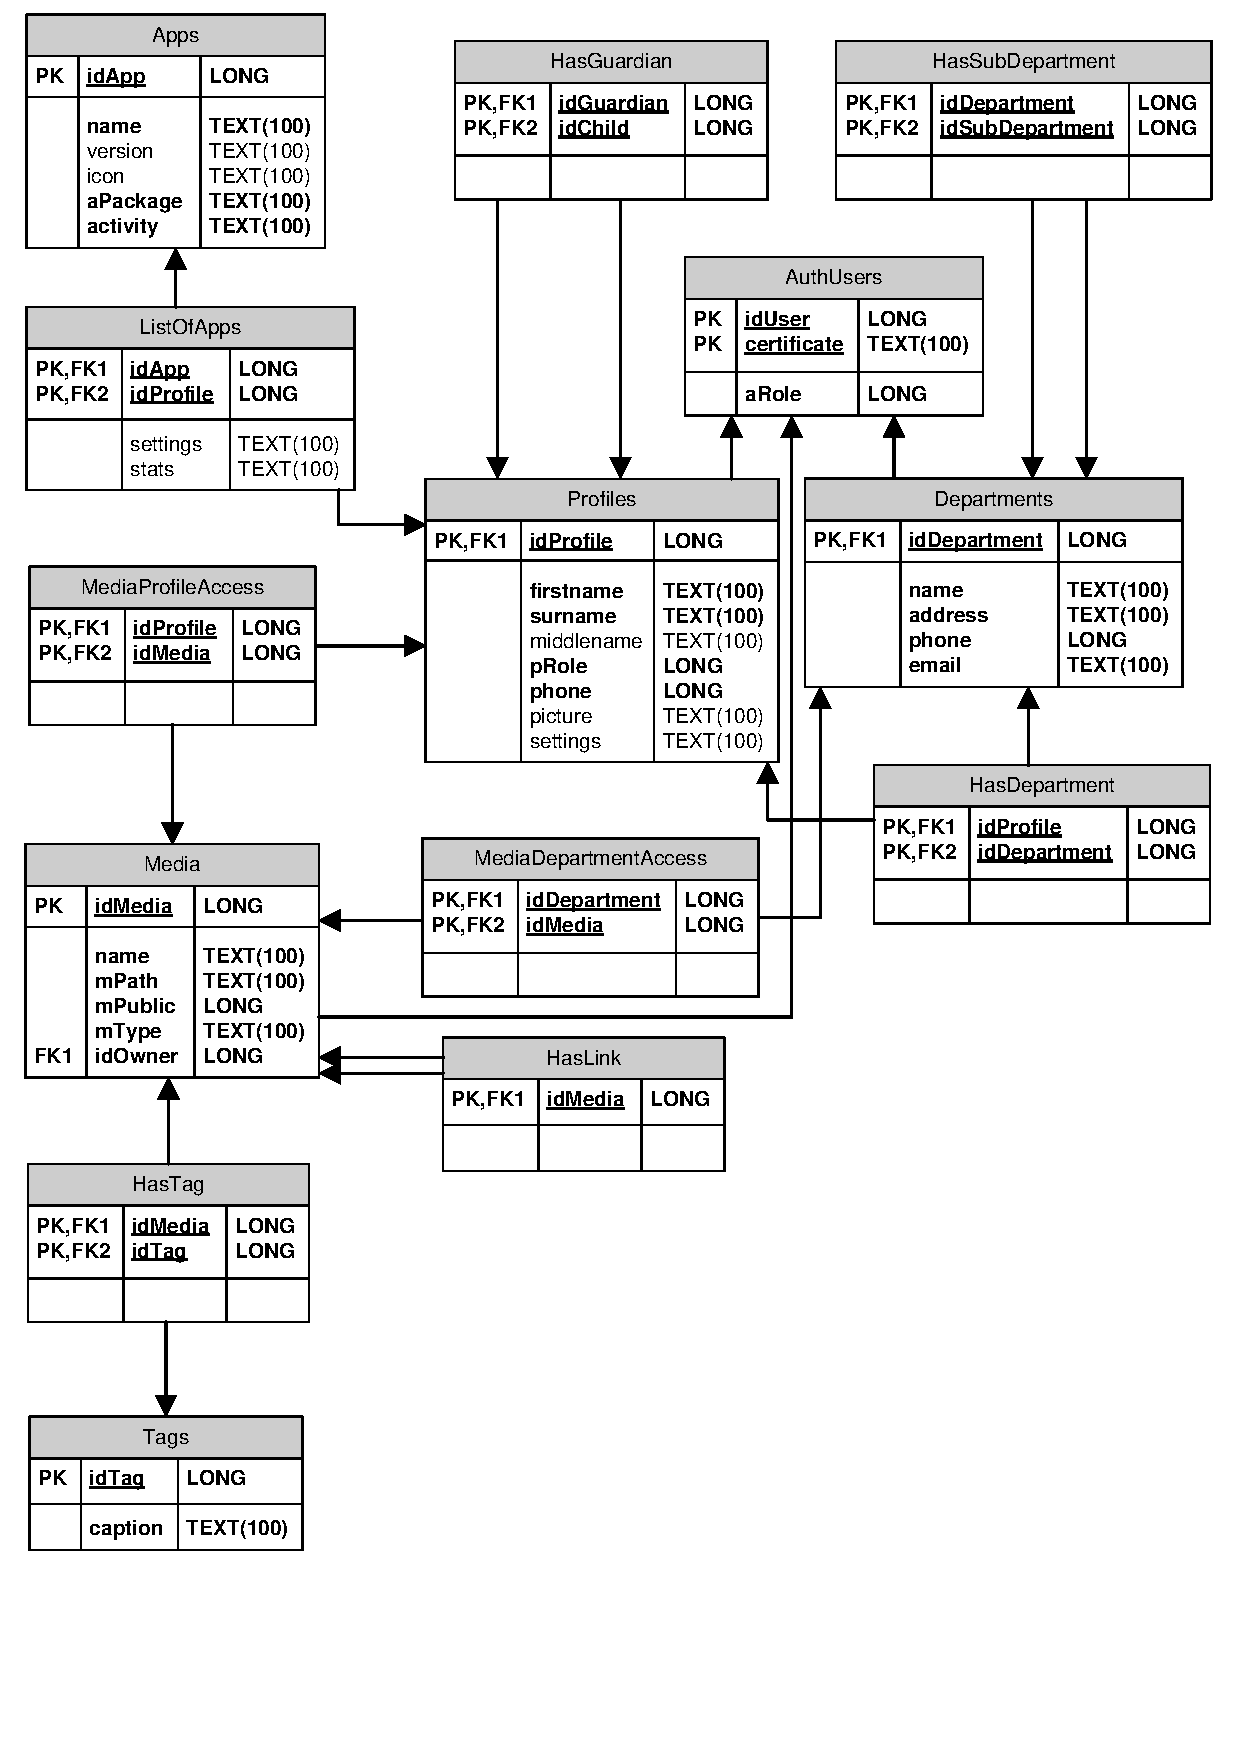
\includegraphics[width=\textwidth]{Images/LocalDatabaseDesign}
	\caption{The schema for the Oasis Local Db.}
	\label{fig:localDatabaseDesign}
\end{figure}

\section{Structure}
\label{sec:OasisStructure}
When using the Android system to develop databases the developers are bound to use the open source database SQLite. \cite{SQLite}
The reason for this is that only SQLite is supported on the Android platform. \cite{AndroidArchitecture}
It supports three kinds of data types; TEXT, which is similar to String type in Java, INTEGER, which is similar to long type in Java, and REAL, which is similar to double type in Java. \cite{SQLTypes}
SQLite does not validate if the types written to the columns actually are of the defined type.
This means that it for instance is possible to write an integer into a TEXT column.
On the positive site SQLite only requires a little portion of memory at runtime. \cite{SQLAbout} 

\section{Implementation}
\label{sec:dbImp}
As stated in Section \vref{sec:OasisStructure}, we implemented the Oasis Local Db using SQLite.
The Oasis Local Db consists of three elements: Metadata, tables, and a content provider.
These are explained in the following sections.

\subsection{Metadata}
First we created metadata files for each table in the Oasis Local Db.

As an example the metadata file for the \texttt{AuthUsers} table can be seen in listing \vref{lst:metadata}.

\begin{Java}{The AuthUsers MetaData}{lst:metadata}
package dk.aau.cs.giraf.oasis.localdb;
import android.net.Uri;
import android.provider.BaseColumns;

public class AuthUsersMetaData {

	public static final Uri CONTENT_URI = Uri.parse("content://dk.aau.cs.giraf.oasis.localdb.AutismProvider/authusers");

	.
	.
	.
	
	public class Table implements BaseColumns {
		public static final String TABLE_NAME = "tbl_authusers";

		public static final String COLUMN_ID = "_id";
		public static final String COLUMN_CERTIFICATE = "authusers_certificate";
		public static final String COLUMN_ROLE = "authusers_role";
	}
}
\end{Java}

In the \texttt{AuthUsers} metadata file the uri, \texttt{CONTENT\_URI}, is used to defined which table to alter. 
The inner class Table defines the strings, which are used as names of the table and the columns.

\subsection{Table}
When the metadata file is created we make a table class file, which defines the SQL statements for creating, updating and deleting the table. The table class file for \texttt{AuthUsers} can be seen in listing \vref{lst:table}.

\begin{Java}{The AuthUsers Table}{lst:table}
package dk.aau.cs.giraf.oasis.localdb;
import android.database.sqlite.SQLiteDatabase;

public class AuthUsersTable {

	private static final String TABLE_CREATE = "CREATE TABLE "
			+ AuthUsersMetaData.Table.TABLE_NAME
			+ "("
			+ AuthUsersMetaData.Table.COLUMN_ID + " INTEGER NOT NULL, "
			+ AuthUsersMetaData.Table.COLUMN_CERTIFICATE + " TEXT NOT NULL, "
			+ AuthUsersMetaData.Table.COLUMN_ROLE + " INTEGER NOT NULL, "
			+ "PRIMARY KEY (" + AuthUsersMetaData.Table.COLUMN_ID + ", " + AuthUsersMetaData.Table.COLUMN_ID + ")"
			+ ");";

	private static final String TABLE_DROP= "DROP TABLE IF EXISTS " + AuthUsersMetaData.Table.TABLE_NAME + ";";

	public static void onCreate(SQLiteDatabase db) {
		db.execSQL(TABLE_CREATE);
	}

	public static void onUpgrade(SQLiteDatabase db, int oldVersion, int newVersion) {
		db.execSQL(TABLE_DROP);
		onCreate(db);
	}
}
\end{Java}

\subsection{Content Provider}
\label{sec:contentProvider}
After the metadata and the tables for the Oasis Local Db has been created, a content provider is created.
The content provider implemented in the Oasis Local Db allow applications to store and retrieve data from the aforementioned tables.

The content provider must implement several methods. These methods are presented along with a code snippet with AuthUsers as an example in the following bullets:

\begin{itemize}
	\item \texttt{onCreate()} - called at startup to initialize the content provider see Listing \vref{lst:onCreate}.
		
		\begin{Java}{The \texttt{onCreate()} method.}{lst:onCreate}
			public boolean onCreate() {
				dbHelper = new DbHelper(getContext());
				return false;
			}
		\end{Java}
	
	\item \texttt{getType()} - called when an application needs to know the type of the data. The \texttt{getType()} method can be seen in Listing \vref{lst:getType}. This method is not used in Oasis Local Db.
		
		\begin{Java}{The \texttt{getType()} method.}{lst:getType}
			public String getType(Uri uri) {
				switch(sUriMatcher.match(uri)) {
				.
				.
				.
				case AUTHUSERS_TYPE_LIST:
					return AuthUsersMetaData.CONTENT_TYPE_AUTHUSERS_LIST;
				case AUTHUSERS_TYPE_ONE:
					return AuthUsersMetaData.CONTENT_TYPE_AUTHUSER_ONE;
				.
				.
				.
				default:
					throw new IllegalArgumentException("Unknown URI: " + uri);
				}
			}
		\end{Java}
	
	\item \texttt{query()} - called when an application wants to query in the Oasis Local Db. The \texttt{query} method can be seen in Listing \vref{lst:query}.
		
		\begin{Java}{The \texttt{query()} method.}{lst:query}
			public Cursor query(Uri uri, String[] projection, String selection, String[] selectionArgs, String sortOrder) {
				SQLiteQueryBuilder builder = new SQLiteQueryBuilder();
				switch(sUriMatcher.match(uri)) {
				.
				.
				.
				case AUTHUSERS_TYPE_LIST:
					builder.setTables(AuthUsersMetaData.Table.TABLE_NAME);
					builder.setProjectionMap(authusersProjectionMap);
					break;
				case AUTHUSERS_TYPE_ONE:
					builder.setTables(AuthUsersMetaData.Table.TABLE_NAME);
					builder.setProjectionMap(authusersProjectionMap);
					builder.appendWhere(AuthUsersMetaData.Table.COLUMN_ID + " = " + uri.getPathSegments().get(1));
					break;
				.
				.
				.
				default:
					throw new IllegalArgumentException("Unknown URI: " + uri);
				}
				SQLiteDatabase db = dbHelper.getReadableDatabase();
				Cursor queryCursor = builder.query(db, projection, selection, selectionArgs, null, null, null);
				queryCursor.setNotificationUri(getContext().getContentResolver(), uri);
				return queryCursor;
			}
		\end{Java}
		
	\item \texttt{insert()} - called when an application wants to insert data into the Oasis Local Db. The \texttt{insert()} method can be seen in Listing \vref{lst:insert}.
	
		\begin{Java}{The \texttt{insert()} method.}{lst:insert}
			public Uri insert(Uri uri, ContentValues values) {
				SQLiteDatabase db = dbHelper.getWritableDatabase();
				long rowId;
				Uri _uri;

				switch(sUriMatcher.match(uri)) {
				.
				.
				.
				case AUTHUSERS_TYPE_LIST:
					try {
						rowId = db.insertOrThrow(AuthUsersMetaData.Table.TABLE_NAME, null, values);
						_uri = ContentUris.withAppendedId(AuthUsersMetaData.CONTENT_URI, rowId);
						getContext().getContentResolver().notifyChange(_uri, null);
					} catch (SQLiteConstraintException e) {
						_uri = ContentUris.withAppendedId(AuthUsersMetaData.CONTENT_URI, -1);
					}
					return _uri;
				.
				.
				.
				default:
					throw new IllegalArgumentException("Unknown URI: " + uri);
				}
			}
		\end{Java}
	
	\item \texttt{update()} - called when an application wants to update existing data in the Oasis Local Db. The \texttt{update()} method can be seen in Listing \vref{lst:update}.
	
		\begin{Java}{The \texttt{update()} method.}{lst:update}
			public int update(Uri uri, ContentValues values, String where, String[] whereArgs) {
				SQLiteDatabase db = dbHelper.getWritableDatabase();
				int rowsUpdated = 0;
				String rowId;

				switch(sUriMatcher.match(uri)) {
				.
				.
				.
				case AUTHUSERS_TYPE_LIST:
					rowsUpdated = db.update(AuthUsersMetaData.Table.TABLE_NAME, values, where, whereArgs);
					break;
				case AUTHUSERS_TYPE_ONE:
					rowId = uri.getPathSegments().get(1);
					rowsUpdated = db.update(AuthUsersMetaData.Table.TABLE_NAME,
							values,
							AuthUsersMetaData.Table.COLUMN_ID + " = " + rowId + (!TextUtils.isEmpty(where) ? " AND (" + where + ")" : ""),
							whereArgs);
					break;
				.
				.
				.
				default:
					throw new IllegalArgumentException("Unknown URI: " + uri);
				}

				getContext().getContentResolver().notifyChange(uri, null);
				return rowsUpdated;
			}
		\end{Java}
	
	\item \texttt{delete()} - called when an application wants to delete existing data in the Oasis Local Db. The \texttt{delete()} method can be seen in Listing \vref{lst:delete}.
	
		\begin{Java}{The \texttt{delete()} method.}{lst:delete}
			public int delete(Uri uri, String where, String[] whereArgs) {
				SQLiteDatabase db = dbHelper.getWritableDatabase();
				int rowsDeleted = 0;
				String rowId;
				.
				.
				.
				case AUTHUSERS_TYPE_LIST:
					rowsDeleted = db.delete(AuthUsersMetaData.Table.TABLE_NAME, where, whereArgs);
					break;
				case AUTHUSERS_TYPE_ONE:
					rowId = uri.getPathSegments().get(1);
					rowsDeleted = db.delete(AuthUsersMetaData.Table.TABLE_NAME,
							AuthUsersMetaData.Table.COLUMN_ID + " = " + rowId + (!TextUtils.isEmpty(where) ? " AND (" + where + ")" : ""),
							whereArgs);
					break;
				.
				.
				.	
				default:
					throw new IllegalArgumentException("Unknown URI: " + uri);
				}

				getContext().getContentResolver().notifyChange(uri, null);
				return rowsDeleted;
			}
		\end{Java}
\end{itemize}

The implemented methods in the content provider supply the functionality for the Oasis Local Db. 
This functionality can be utilized in the implementation of the Oasis Lib.